\problemname{Opstilling}
En gruppe med $n$ børn, lad os kalde dem A, B, C osv., har besluttet sig for at stille dine tankeevner på prøve.
Du lukker øjnene, og børnene stiller sig på række.
Så tæller hvert barn antallet af større børn til hhv. venstre og højre for sig selv.
Hvert barn skriver disse to tal på en seddel, som du modtager efter at børnene har forladt opstillingen, og du har åbnet øjnene igen.
Børnenes opgave til dig er at finde ud af, i hvilken rækkefølge de stod.

Et eksempel med fem børn er vist i figuren.
A har et større barn (D) til venstre og to større børn (C og E) til højre.
B har tre større børn til venstre og et til højre.
C har et større børn til venstre men ingen til højre. 
Informationen på sedlerne kan sammenfattes således:

\begin{figure}[h!]
  \centering

\begin{minipage}{.5\textwidth}
    \begin{tabular}[b]{|c|c|c|}
    \hline
      Barn&Venstre&Højre\\\hline
      A&1&2\\
      B&3&1\\
      C&1&0\\
      D&0&0\\
      E&2&0\\\hline
    \end{tabular}
\end{minipage}%
\begin{minipage}{.5\textwidth}
    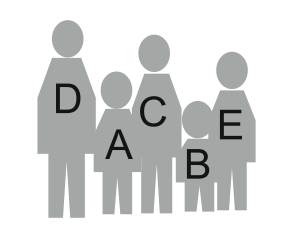
\includegraphics[scale=0.4]{uppstallning.png}
\end{minipage}

\end{figure}

Desværre er opgaven alt for svær for dig, så du er nødt til i hemmelighed at skrive et program til at løse opgaven.
For at gøre det nemmere for dig næste gang du møder børnene, vil du kunne variere både antallet af børn (mellem $3$ og $8$, inklusive) og informationen på sedlerne.
Du kan gå ud fra, at børnene er af forskellig højde og at sedlerne er udfyldt korrekt.
Interessant nok er løsningen entydigt bestemt.

\section*{Indlæsning}
Første linje består af et heltal $n$ ($3 \le n \le 8$), antallet af børn.
Derefter følger $n$ linjer, en for hvert barn,  med to heltal på hver: antallet af større børn til venstre og antallet af større børn til højre.

\section*{Udskrift}
Skriv en enkelt linje med $n$ tegn, som beskriver børnenes opstilling, som en permutation af \texttt{A}, \texttt{B}, \texttt{C} osv.
